\documentclass{article}
\usepackage{mathtools} 
\usepackage{fontspec}
\usepackage[UTF8]{ctex}
\usepackage{amsthm}
\usepackage{mdframed}
\usepackage{xcolor}
\usepackage{amssymb}
\usepackage{amsmath}
\usepackage{tikz}
\usepackage{pgfplots}
\usepgfplotslibrary{polar}
% \pgfplotsset{compat=1.18}


% 定义新的带灰色背景的说明环境 zremark
\newmdtheoremenv[
  backgroundcolor=gray!10,
  % 边框与背景一致，边框线会消失
  linecolor=gray!10
]{zremark}{说明}

% 通用矩阵命令: \flexmatrix{矩阵名}{元素符号}{行数}{列数}
\newcommand{\flexmatrix}[4]{
  \[
  #1 = \begin{pmatrix}
    #2_{11}     & #2_{12}     & \cdots & #2_{1#4}   \\
    #2_{21}     & #2_{22}     & \cdots & #2_{2#4}   \\
    \vdots      & \vdots      & \ddots & \vdots     \\
    #2_{#31}    & #2_{#32}    & \cdots & #2_{#3#4}
  \end{pmatrix}
  \]
}

% 简化版命令（默认矩阵名为A，元素符号为a）: \quickmatrix{行数}{列数}
\newcommand{\quickmatrix}[2]{\flexmatrix{A}{a}{#1}{#2}}

\begin{document}
\title{习题 10.1}
\author{张志聪}
\maketitle

\section*{4}

方法1：四个图形的面积之和，证明略。


方法2（三角函数推荐）：利用变量替换，函数的奇偶性。

按封闭曲线计算公式
\begin{align*}
  A & = \left|\int_{\alpha}^{\beta} y(t) x'(t) dt \right|              \\
    & = \left|\int_{0}^{2\pi} a sin^3 t (- 3a cos^2 t sint dt) \right| \\
    & = \left|- 3a^2\int_{0}^{2\pi} sin^4 t cos^2 t dt \right|         \\
    & = 3a^2 \left|\int_{0}^{2\pi} sin^4 t cos^2 t dt \right|          \\
\end{align*}
令$u = t - \pi, t: 0 \to 2\pi, u: -\pi \to \pi, dt = du$，于是
\begin{align*}
  \int_{0}^{2\pi} sin^4 t cos^2 t dt
   & = \int_{-\pi}^{\pi} sin^4 (u + \pi) cos^2(u + \pi) du \\
   & = \int_{-\pi}^{\pi} sin^4 (u + \pi) cos^2(u + \pi) du \\
   & = \int_{-\pi}^{\pi} sin^4 u cos^2u du
\end{align*}
因为$sinu$是奇函数，所以$sin^4u$是偶函数，$cosu$是偶函数，所以$cos^2u$是偶函数，
于是$sin^4 u cos^2u$是偶函数。我们有
\begin{align*}
  \int_{-\pi}^{\pi} sin^4 u cos^2u du
   & = 2 \int_{0}^{\pi} sin^4 u cos^2u du
\end{align*}
令$z = u - \frac{\pi}{2}, u: 0 \to \pi, z: -\frac{\pi}{2} \to \frac{\pi}{2}, du = dz$，
\begin{align*}
  \int_{0}^{\pi} sin^4 u cos^2u du
   & = \int_{-\frac{\pi}{2}}^{\frac{\pi}{2}} sin^4 (z + \frac{\pi}{2}) cos^2(z + \frac{\pi}{2}) dz \\
   & = \int_{-\frac{\pi}{2}}^{\frac{\pi}{2}} cos^4 z sin^2z dz
\end{align*}
类似地，$cos^4 z sin^2z$是偶函数，我们有
\begin{align*}
  \int_{-\frac{\pi}{2}}^{\frac{\pi}{2}} cos^4 z sin^2z dz
   & = 2 \int_{0}^{\frac{\pi}{2}} cos^4 z sin^2z dz
\end{align*}
综上，
\begin{align*}
  3a^2 \left|\int_{0}^{2\pi} sin^4 t cos^2 t dt \right|
   & = 3a^2 \left| 4 \int_{0}^{\frac{\pi}{2}} cos^4 z sin^2z dz \right| \\
   & = 12a^2 \left| \int_{0}^{\frac{\pi}{2}} cos^4 z sin^2z dz \right|
\end{align*}
由第九章$\S 5$习题8可知
\begin{align*}
  J(4,2) & = \frac{1}{2}J(2, 2)                         \\
         & = \frac{1}{2} \frac{1}{4}J(0, 2)             \\
         & = \frac{1}{2} \frac{1}{4} \frac{1}{2}J(0, 0) \\
         & = \frac{1}{16} \frac{\pi}{2}                 \\
         & = \frac{\pi}{32}
\end{align*}
所以
\begin{align*}
  12a^2 \left| \int_{0}^{\frac{\pi}{2}} cos^4 z sin^2z dz \right|
   & = 12a^2 \frac{\pi}{32} \\
   & = \frac{3}{8} a^2 \pi
\end{align*}

\section*{5}
\begin{tikzpicture}
  \begin{polaraxis}[
      grid=both,
      minor tick num=1,
      title={$r = 1(1 + cos(x))$，以$a=1$为例},
    ]
    \addplot[domain=0:360, samples=400, thick, blue] {1(1 + cos(x))};
  \end{polaraxis}
\end{tikzpicture}

极坐标的面积：
\begin{align*}
  A & = \frac{1}{2} \int_{0}^{2\pi} r^2(\theta) d \theta                                                                                   \\
    & = \frac{1}{2} \int_{0}^{2\pi} a^2(1 + cos\theta)^2 d \theta                                                                          \\
    & = \frac{a^2}{2} \int_{0}^{2\pi} 1 + cos^2\theta + 2 cos\theta d \theta                                                               \\
    & = \frac{a^2}{2} \left[\int_{0}^{2\pi} 1 d\theta + \int_{0}^{2\pi} cos^2\theta d\theta + 2 \int_{0}^{2\pi} cos\theta d \theta \right] \\
    & = \frac{a^2}{2} \left[2\pi + \int_{0}^{2\pi} \frac{1}{2}(1 + cos2\theta) d\theta + 2 sin\theta \bigg|_0^{2\pi} \right]               \\
    & = \frac{a^2}{2} \left[2\pi + \frac{1}{2}(x + \frac{1}{2}sin2\theta)\bigg|_0^{2\pi} + 0 \right]                                       \\
    & = \frac{a^2}{2} \left[2\pi + \pi + 0\right]                                                                                          \\
    & = \frac{3}{2}a^2 \pi
\end{align*}

\section*{6}

\begin{tikzpicture}
  \begin{polaraxis}[
      grid=both,
      minor tick num=1,
      title={$r = 1\sin(3\theta)$，以$a=1$为例},
    ]
    \addplot[domain=0:360, samples=400, thick, blue] {1*sin(3*x)};
  \end{polaraxis}
\end{tikzpicture}

通过画图过程可知积分上下限为$0 \to \pi$（注：直接看图是看不出来的）。

\begin{align*}
  A & = \frac{1}{2} \int_{0}^{\pi} r^2(\theta) d \theta                    \\
    & = \frac{1}{2} \int_{0}^{\pi} r^2(\theta) d \theta                    \\
    & = \frac{1}{2} \int_{0}^{\pi} a^2sin^2 3\theta d \theta               \\
    & = \frac{a^2}{2} \int_{0}^{\pi} \frac{1}{2}(1 - cos 6\theta) d \theta \\
    & = \frac{a^2}{4} \int_{0}^{\pi} 1 - cos 6\theta d \theta              \\
    & = \frac{a^2}{4} (x - \frac{1}{6}sin 6 \theta)\bigg|_0^{\pi}          \\
    & = \frac{a^2}{4} \pi
\end{align*}

\textcolor{red}{注：玫瑰线}
\begin{align*}
  r = a sin n \theta (a > 0)
\end{align*}
当$n$为奇数，闭合周期$\pi$；\\
当$n$为偶数，闭合周期$2\pi$.

\section*{7}

显然$x: 0 \to a$，否则等式不成立。

计算$y$关于$x$的表达式:
\begin{align*}
  \sqrt{\frac{x}{a}} + \sqrt{\frac{y}{b}} & = 1                                        \\
  \sqrt{\frac{y}{b}}                      & = 1 - \sqrt{\frac{x}{a}}                   \\
  \frac{y}{b}                             & = 1 + \frac{x}{a} - 2\sqrt{\frac{x}{a}}    \\
  y                                       & = b + \frac{b}{a} x - 2b\sqrt{\frac{x}{a}}
\end{align*}
于是，面积为
\begin{align*}
  A & = \int_0^{a} b + \frac{b}{a} x - 2b\sqrt{\frac{x}{a}} dx                              \\
    & = (bx + \frac{b}{2a}x^2 - \frac{2b}{\sqrt{a}} \frac{2}{3}x^{\frac{3}{2}})\bigg|_0^{a} \\
    & = (bx + \frac{b}{2a}x^2 - \frac{4b}{3\sqrt{a}} x^{\frac{3}{2}})\bigg|_0^{a}           \\
    & = ab + \frac{1}{2}ab - \frac{4}{3} ab - 0                                             \\
    & = \frac{1}{6}ab
\end{align*}

\section*{8}

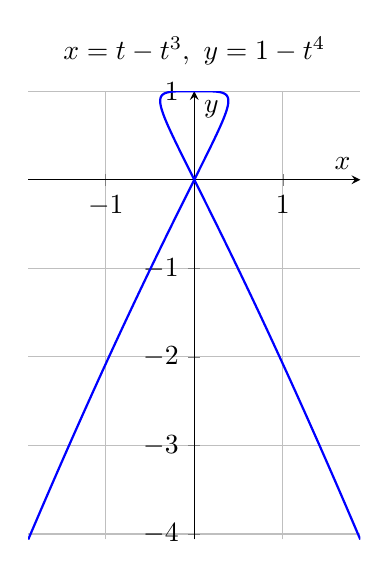
\begin{tikzpicture}
  \begin{axis}[
      axis lines=middle,      % 坐标轴穿过原点
      grid=both,              % 显示网格
      xlabel=$x$, ylabel=$y$,
      title={$x = t - t^3,\ y = 1 - t^4$},
      samples=400,
      domain=-1.5:1.5,
      axis equal image,       % 保持比例一致
    ]

    \addplot[
      parametric,
      thick,
      blue,
    ]
    ({x - x^3}, {1 - x^4});
  \end{axis}
\end{tikzpicture}

为什么这么画：
https://www.bilibili.com/video/BV1jW4y1S7z5?t=476.0\&p=153

因为$x(-1) = x(1)$，于是
\begin{align*}
  A & = \left| \int_{-1}^{1} y(t) x'(t)  dt\right|        \\
    & = \left| \int_{-1}^{1} (1- t^4)(1 - 3t^2) dt\right| \\
    & = \frac{16}{35}
\end{align*}

\section*{9}

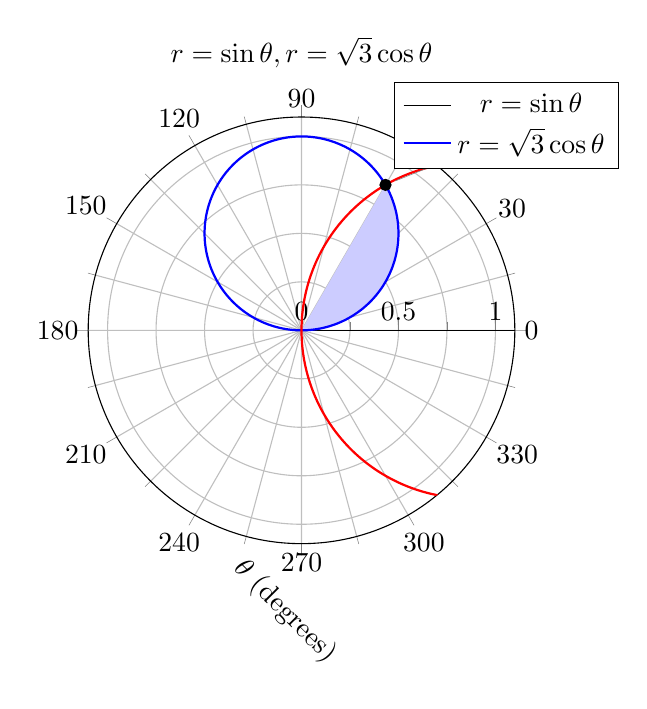
\begin{tikzpicture}
  \begin{polaraxis}[
      title={$r=\sin\theta, r=\sqrt{3}\cos\theta$ },
      grid=both,
      minor tick num=1,
      axis equal image,
      ymin=0, ymax=1.1,             % 显示半径范围（可调）
      xlabel style={at={(axis description cs:0.5,-0.12)},anchor=north},
      xlabel={$\theta$ (degrees)},
      width=7cm,
      height=7cm,
    ]

    % 填充公共部分（theta 从 0 到 60 度，填充到 origin）
    \addplot[
      domain=0:60,
      samples=200,
      draw=none,
      fill=blue!20
    ] {sin(x)};            % 在 polaraxis 环境中，addplot {r} 的填充默认填到 r=0

    % 绘出 r = sin(theta)
    \addplot[
      domain=0:360,
      samples=400,
      thick,
      blue
    ] {sin(x)};
    \addlegendentry{$r=\sin\theta$}

    % 绘出 r = sqrt(3) cos(theta)
    \addplot[
      domain=0:360,
      samples=400,
      thick,
      red
    ] {sqrt(3)*cos(x)};
    \addlegendentry{$r=\sqrt{3}\cos\theta$}

    % 在交点处做一个标记（theta = 60 deg, r = sin(60)）
    \addplot[only marks, mark=*, mark options={fill=black}, samples=1] coordinates {(60, {sin(60)})};

    % 可选：标注交点坐标
    \node[black, font=\small] at (axis cs:60, {sin(60)}) [pin=45:{$(\,r=\tfrac{\sqrt3}{2},\ \theta=60^\circ\,)$}] {};

  \end{polaraxis}
\end{tikzpicture}

对工具绘图用的不太好，右边的圆没有显示完整。

两个极坐标曲线的交点为
\begin{align*}
  sin \theta & = \sqrt{3}cos \theta \\
  tan \theta & = \sqrt{3}           \\
  \theta     & = \frac{\pi}{3}
\end{align*}
公共部分是两个部分的和
\begin{align*}
  A & = \frac{1}{2} \int_0^{\frac{\pi}{3}} (sin \theta)^2 d\theta + \frac{1}{2} \int_{\frac{\pi}{3}}^{\frac{\pi}{2}} (\sqrt{3}cos \theta)^2 d\theta              \\
    & = \frac{1}{2} \int_0^{\frac{\pi}{3}} sin^2 \theta d\theta + \frac{1}{2} \int_{\frac{\pi}{3}}^{\frac{\pi}{2}} 3cos^2 \theta d\theta                         \\
    & = \frac{1}{4} \int_0^{\frac{\pi}{3}} (1 - cos2\theta) d\theta + \frac{3}{4} \int_{\frac{\pi}{3}}^{\frac{\pi}{2}} (1 + cos2 \theta) d\theta                 \\
    & = \frac{1}{4} (\theta - \frac{1}{2}sin2\theta)\bigg|_0^{\frac{\pi}{3}} + \frac{3}{4}(\theta + \frac{1}{2}sin2\theta)\bigg|_{\frac{\pi}{3}}^{\frac{\pi}{2}} \\
    & = \frac{1}{4} (\frac{\pi}{3} - \frac{\sqrt{3}}{4} - 0) + \frac{3}{4}(\frac{\pi}{6} - \frac{\sqrt{3}}{4})                                                   \\
    & = \frac{5\pi}{24} - \frac{\sqrt{3}}{4}
\end{align*}

% \section*{10}

% \begin{align*}
%   \frac{x^2}{a^2} + \frac{y^2}{b^2} & = 1 \\
%   \frac{x^2}{b^2} + \frac{y^2}{a^2} & = 1 
% \end{align*}

\end{document}